\chapter{ESR}
\section{Setup}
\begin{figure}
	\centering
	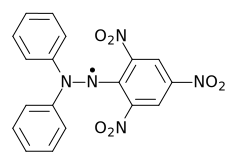
\includegraphics[width=0.5\textwidth]{./img/DPPH.pdf}
	\caption[]{\textbf{2,2-diphenyl-1-picrylhydrazyl (DPPH)} The unpaired electron of the nitrogen radical makes the sample suitable for ESR experiments.}
	\label{fig:DPPH}
\end{figure}
The whole experiment is layed out around a main system which consists of the ESR probe with three interchangable ESR coils, which all cover different frequency ranges.
This ESR probe emits microwaves.

A sample can be inserted into the coils.
In this experiment, an organic compound called DPPH (2,2-diphenyl-1-picrylhydrazyl) is used (\autoref{fig:DPPH}).
DPPH has a distinct ESR spectral line which also acts as a standard in ESR experiments.

The ESR probe is powered by the basic device which also contains a frequency gauge.
Helmholtz coils (distance between coils: $d=r=\SI{68}{\mm}$), which are used to create an external magnetic field, are powered by an adjustable transformer.
The Zeeman splitting discussed in \autoref{sec:zeeman} is provided by the Helmholtz coils.

Both the ESR probe's signal and the Helmholtz coils' current (using a shunt resistor) are connected to a 2-channel oscilloscope.

\section{Exercise 1: Intro-Experiment}
A passive, resonant circuit consisting of a coil and variable capacitor is mounted next to the ESR probe.
The AC voltage across the variable capacitor is measured with a multimeter while varying the ESR probe's frequency.
However, the multimeter does not provide the bandwidth to carry out such measurements.
Although a miniscule voltage is observed at the multimeter for a specific tuning of the HF frequency, the result is not significant enough.
If a significant voltage had been measured, it would prove that the resonant circuit drained energy from the ESR probe's electromagnetic field.

\section{Exercise 2 and 3: External Field Dependence}
A DPPH-sample is inserted into the ESR probe and an external, sinusoidal magnetic field is generated by a Helmholtz-coil.
The head of the ESR probe is placed at the coil's center to ensure that the field is as homogenous as possible.
The probe's resonance peaks are measured with three different ESR coils.

The maximum magnetic field is varied by changing the voltage amplitude of the Helmholtz coils.
With decreasing amplitude, the peaks in the spectrum drift apart from the modulation signal's zero crossing.
This can be explained by the fact that, for low amplitudes, the resonance field strengths are shifted towards the voltage peak, until resonance is only visible once per period for sufficiently small amplitudes.

Upon removing the sample from the ESR probe, the characteristic spectrum vanishes.
This means that the measured peaks actually originate from the sample's resonance.
Increasing the HF amplitude of the ESR probe increases the signal strength in the spectrum.
This behavior can be explained by the increasing number of spins that are excited inside of the sample.
Hence, for extraordinarily high amplitudes the signal strength should reach a saturation point.
This behavior cannot be observed as the amplitude available is limited by the ESR probe.

\section{Exercise 4: Measuring the g-Factor}
\subsection{Data}
\begin{table}[tbp]
	\centering
	\caption[g-factor measurement: First coil]{\textbf{g-factor measurement: First coil ($f=13-30\si{\MHz}$)}}
	\label{tab:firstcoil}
	\begin{tabular}{S|SSS}
		\toprule
		{$f$ in \si{\MHz}}	&	{$U_1$ in \si{\mV}}	&	{$U_2$ in \si{\mV}}	&	{$\bar{U}$ in \si{\mV}} \\
		\midrule
		13	 & 	160	 & 	-96.6	&	128.3	\\
		18	 & 	210	 & 	-150	&	180	\\
		23	 & 	257	 & 	-200	&	228.5	\\
		28	 & 	300	 & 	-267	&	283.5	\\
		33	 & 	347	 & 	-307	&	327	\\
		\bottomrule
	\end{tabular}
\end{table}
\begin{table}[tbp]
	\centering
	\caption[g-factor measurement: Second coil]{\textbf{g-factor measurement: Second coil ($f=30-75\si{\MHz}$)}}
	\label{tab:secondcoil}
	\begin{tabular}{S|SSS}
		\toprule
		{$f$ in \si{\MHz}}	&	{$U_1$ in \si{\mV}}	&	{$U_2$ in \si{\mV}}	&	{$\bar{U}$ in \si{\mV}} \\
		\midrule
		70	 & 	720	 & 	-666	&	693	\\
		80	 & 	806	 & 	-753	&	779.5	\\
		90	 & 	916	 & 	-866	&	891	\\
		100	 & 	1020	 & 	-966	&	993	\\
		110	 & 	1120	 & 	-1070	&	1095	\\
		120	 & 	1220	 & 	-1170	&	1195	\\
		130	 & 	1320	 & 	-1270	&	1295	\\
		\bottomrule
	\end{tabular}
\end{table}

\begin{table}[tbp]
	\centering
	\caption[g-factor measurement: Second coil]{\textbf{g-factor measurement: Third coil ($f=75-130\si{\MHz}$)}}
	\label{tab:thirdcoil}
	\begin{tabular}{S|SSS}
		\toprule
		{$f$ in \si{\MHz}}	&	{$U_1$ in \si{\mV}}	&	{$U_2$ in \si{\mV}}	&	{$\bar{U}$ in \si{\mV}} \\
		\midrule
		70	 & 	720	 & 	-666	&	693	\\
		80	 & 	806	 & 	-753	&	779.5	\\
		90	 & 	916	 & 	-866	&	891	\\
		100	 & 	1020	 & 	-966	&	993	\\
		110	 & 	1120	 & 	-1070	&	1095	\\
		120	 & 	1220	 & 	-1170	&	1195	\\
		130	 & 	1320	 & 	-1270	&	1295	\\
		\bottomrule
	\end{tabular}
\end{table}

The ESR spectrum is measured for all three coils while varying the HF frequency.
The external magnetic field's amplitude is held at a constant level.
Measured data can be seen in tables \ref{tab:firstcoil}, \ref{tab:secondcoil} and \ref{tab:thirdcoil}.

As discussed in \autoref{sec:esr}, the system has to satisfy the resonance condition.
Rearranging \autoref{eq:resonance}, the g-factor can be determined by fitting the linear model
\begin{equation}\label{eq:gfac}
	\nu=\underbrace{g\frac{\mu_\text{B}}{h}}_a \cdot B,
\end{equation}
to the measured data.

The lab instruction provides the relation between the voltage and magnetic field generated by the Helmholtz coil
\begin{equation}\label{eq:extfield}
	B=\frac{U}{R}\cdot\SI{3.96}{\milli\tesla\per\ampere}.
\end{equation}
The voltage is measured across a \SI{1.07}{\ohm} shunt resistor and is determined by averaging the absolute values of the voltages from both half-waves
\begin{equation*}
	U = \frac{\abs{U_1}+\abs{U_2}}{2}.
\end{equation*}

\subsection{Error Calculation}
Assuming an error of $\Delta U_i=\SI{20}{\mV}$, which complies with 2 LSB of the used oscilloscope, the voltage uncertainty propagates like
\begin{alignat*}{2}
	\Delta U &= \sqrt{\sum^2_{i=1}\left(\pdb{U}{U_i}\cdot \Delta U_i\right)^2} \\
	&=\frac{1}{\sqrt{2}}\Delta U_i,
\end{alignat*}
which translates into the error of the magnetic field as
\begin{alignat*}{2}
	\Delta B &= \abs{\pdb{B}{U}}\cdot \abs{\Delta U_i} \\
	&= \frac{\SI{3.96}{\milli\tesla\per\ampere}}{\sqrt{2}R}\cdot\Delta U_i \\
	&= \SI{52.3}{\micro\tesla}.
\end{alignat*}

The uncertainty of the ESR frequency can be estimated as $\Delta\nu = \SI{100}{\kHz}$, which is the resolution of the used frequency counter.

Rearranging the term for the slope in \autoref{eq:gfac}, the error of the slope coefficient aquired by the linear fit propagates into the g-factor like
\begin{alignat*}{2}
	\Delta g_i &= \abs{\pdb{g}{a}}\cdot \abs{\Delta a_i} \\
	&= \frac{h}{\mu_\text{B}}\cdot\Delta a_i.
\end{alignat*}

Averaging over the different g-factors also generates a statistical error of
\begin{equation*}
	\sigma_g = \frac{\sigma_{g_i}}{\sqrt{N=3}}.
\end{equation*}

Additionally, the errors from previously calculated values propagate into their mean value as
\begin{equation*}
	\Delta g = \sqrt{\frac{1}{N}\sum_{i=1}^3 \left(\Delta g_i\right)^2}.
\end{equation*}

\subsection{Results}
\begin{figure}[!htb]
	\minipage{0.5\textwidth}
		\includegraphics[width=\linewidth]{./data/plots/coilE.pdf}
		\caption*{Linear fit for Coil E ($f=13-30\si{\MHz}$)}\label{fig:coilE}
	\endminipage\hfill
	\minipage{0.5\textwidth}
	\includegraphics[width=\linewidth]{./data/plots/coilF.pdf}
	\caption*{Linear fit for Coil F ($f=30-75\si{\MHz}$)}\label{fig:coilF}
	\endminipage\hfill\centering
	\minipage{0.5\textwidth}%
	\includegraphics[width=\linewidth]{./data/plots/coilG.pdf}
	\caption*{Linear fit for Coil G ($f=75-130\si{\MHz}$)}\label{fig:coilG}
	\endminipage
	\caption[Linear fits for all ESR coils]{\textbf{Linear fits for all ESR coils} The linear behavior is proven for all three frequency ranges with a coefficient of determination $R^2=\num{99.9}\%$}
	\label{fig:allcoils}
\end{figure}

Linear fits for all three ESR coils can be seen in \autoref{fig:allcoils}.
As expected, there is a linear dependence between the HF frequency $f$ and the resonant magnetic field strength $B$.
Using the determined slopes, the g-factors are calculated as
\begin{alignat*}{3}
	g &= \frac{a\cdot h}{\mu_\text{B}} \\
	&= \num{1.93(17)}\qquad\text{with } a_\text{E}&=\SI{26.95(241)}{\MHz\per\milli\tesla} \\
	&= \num{1.88(5)}\qquad\text{with } a_\text{F}&=\SI{26.37(71)}{\MHz\per\milli\tesla} \\
	&= \num{1.90(5)}\qquad\text{with } a_\text{G}&=\SI{26.62(70)}{\MHz\per\milli\tesla}.
\end{alignat*}

Averaging these values gives the final result of
\begin{equation*}
	g = \num{1.903}\pm\num{0.015}\ \text{(stat.)}\pm\num{0.11}\ \text{(sys.)}.
\end{equation*}

This result is in compliance with the literature value $g_\text{lit}%it's lit yo
=\num{2.0036}$\cite{g-factor}.
